% Co udělal někdo jinej
\chapter{Rešerše ($\sum$ = 9 stran)} \label{chap:Rešerše}
\section{Frekvenční měniče a jejich role v řízení dopravníků (6,5 stran)}\label{sec:FrekvencniMeniceAJejichRole}
%\purpose{Vysvětlit s jakým systémem už pracuji}

Dopravníkové systémy byly kdysi pouze robustní mechanické konstrukce s jednoduchým asynchronním motorem napojený na jednu hodnotu síťového napětí a s nemotornou regulací rychlosti například pomocí přidáním odporu do sekundárního vinutí. V dnešní době jsme v éře průmyslu 4.0. a s tím je v každém mechatronickém systému důraz na automatizaci a digitalizaci spojených procesů. Díky velkému pokroku v oblasti výkonové elektrotechniky a řídících systémů vznikly nové možnosti precizního řízení otáček asynchronních motorů. Důležitým prvkem této transformace se staly frekvenční měniče - zařízení které umí na vstupu brát síťové napětí a na výstupu poskytovat jinou amplitudu a frekvenci napětí, což umožňuje efektivně řídit otáčky jakýchkoliv asynchronních motorů. Tohle umožnilo vznik dopravníkových systémů u kterých je možné přesně a efektivně řídit otáčky. Když se k tomuto systému přidají ještě řídící systémy, je možné znát v každé chvíli polohu balíků na lince a inteligentně tento tok balíků řídit.

Dopravníkové systémy, které společnost Honeywell vytváří jsou přesně takové inteligentní dopravníkové systémy. Cílem těchto systémů je pro zákazníky (většinou dopravní společnosti nebo například supermarkety) vytvořit systém, na který stačí vložit balík na jednom místě a tento balík už doputuje na místo kde má skončit. Řídící systém se postará o zbytek činností jako je třeba naskenování QR kódu na balíku, identifikace koncového bodu a řízení všech linek tak, aby nedošlo ke kolizím nebo nebezpečným událostem.

V současné době jsou tyhle jednotlivé dopravníky poháněné třífázovými asynchronními motory, které pomocí složitých převodů roztáčí celý dopravník (všechny jeho válečky nebo pás). Tyhle asynchronní motory jsou poháněné frekvenčními měniči a ty jsou pro většinu Honeywell dopravníkových systémů v dnešní době model G120D od značky Sinamics. Frekvenční měnič poskytuje výstup do asynchronního motoru, ale jedná se pouze o výkonovou část. Aby bylo možné frekvenční měnič řídit, je potřeba na něj připojit i ovládací panel, které je v běžné sestavě Honeywell dopravníkových systémů model CU240D-2 od značky Sinamics. Při běžném provozu je na tenhle ovládací panel připojená komunikační sběrnice PROFINET, která dává frekvenčnímu měniči ovládací příkazy. PROFINET je naprogramovaný přes Siemens TIA Portal (Total Integrated Automation Portal), což je prostředí vyvinuté od Siemens právě pro řízení různých frekvenčních měničů pomocí Siemens programovatelných logických automatů (PLC). V tomto programu je modelovaný tok na lince a pomocí toho PLC automaticky řídí dopravníkový systém.
\cite{SinamicsG120D}

Zařízení, které v je v této bakalářské práci navrženo se ale nekoncipuje pro standardní provoz dopravníkových systémů, protože tam je systém už řízený PLC. Tento systém je navrhovaný pro zjednodušení procesu kontroly kvality instalace a funkčnosti dopravníků, který je konaný hned po instalaci dopravníků (které instaluje externí firma) v prostorách zákazníků. Jedná se hlavně o dynamické kontroly kvality mechanické instalace, kdy se na každém dopravníku musí zkontrolovat, že je schopný pohybu bez přílišného házení nebo vibrací kvůli špatné instalaci.

V kontextu těchto zkoušek není nezbytné, aby frekvenční měniče komunikovaly prostřednictvím řídicího systému Siemens PLC. Opak je pravdou - zde je inicializace PLC sítě mezi dopravníky spíše extra úkol, což jsou schopnosti které často zaměstnanci kontrolující mechanickou instalaci dopravníků nemají. Při těchto zkouškách se stává prioritní mít kontrolu nad individuálními dopravníky a mít možnost je ovládat a nastavovat na nich rychlost dle libosti. Výhodou by zde při takovém ovládání byla i možnost implementace dálkového ovládání dopravníků.

\subsection{Jak frekvenční měniče fungují}\label{sec:JakFungujiFrekvencniMenice}
%\purpose{Vysvětlit jak vlastně ten frekvenční měnič funguje a proč ho používáme v dopravnících}

Jak již bylo naznačeno v kapitole \ref{sec:FrekvencniMeniceAJejichRole}, frekvenční měniče se pro řízení asynchronních motorů teoreticky používat nemusí, ale poté by měl dopravník jenom omezený výběr z nastavitelných rychlostí a celé řízení by bylo mnohem složitější. V dnešní době jsou frekvenční měniče technicky nejvýhodnější způsob regulace motorů jak z hlediska technických parametrů (regulační rozsah a přesnost), tak i z energetického hlediska (regulace je bezeztrátová). Kvůli těmto důvodům jsou frekvenční měniče tak časté.  \cite{FrekvencniMeniceZeSkriptElektrickeRegulovanePohony}

Frekvenční měnič Sinamics G120D je sice vektorově řízený, ale princip funkce frekvenčního měniče se dá lépe vysvětlit na měniči se skalárním řízením.

Rozdíl mezi těmito dvěma způsoby řízení spočívá v efektivitě. Vektorové řízení cíleně reguluje proud v cívkách asynchronního motoru tak, aby statorové magnetické pole bylo prostorově optimálně natočené vůči poli rotorovému (úhel závisí na počtu pólů). Díky tomu je dosaženo efektivnějšího pohonu rotoru požadovanou rychlostí a směrem. Skalární řízení naopak tento vzájemný úhel nesleduje, a proto není z hlediska řízení optimální. Vektorové řízení je zkrátka složitější, ale efektivnější a má další výhodu že umožňuje přímé řízení momentu.
\cite{FrekvencniMeniceZeSkriptElektrickeRegulovanePohony}

Funkce frekvenčního měniče vychází přímo z principu funkce asynchronního motoru. Při návrhu asynchronního motoru se navrhuje velikost sycení motoru které je určeno spřaženým magnetickým tokem statorového vinutí $\Psi_S$ který je definován jako:
\begin{equation}
	\Psi_S = N\Phi_S
	\label{eq:SdruzenyMagnetickyTok}
\end{equation}
kde N je počet závitů cívky na statoru a $\Phi_S$ je magnetický tok jednoho závitu cívky.

Aby frekvenční měnič mohl fungovat, musí být spřažený magnetický tok statorového vinutí konstantní. Tomu se říká \textbf{Podmínka konstantního sycení}. Statorové vinutí motoru je napájeno nějakým harmonickým napětím vycházející z frekvenčního měniče o tvaru:
\begin{equation}
	U_S(t) = U_{max}sin(\omega_st)
	\label{eq:NapetiNaStatoru}
\end{equation}
kde $U_S$ je napětí na statoru, $U_{max}$ je amplituda statorového napětí a $\omega_s$ je úhlová frekvence napájecího napětí.
\cite{SkriptaRizeniOtacekAM}

Pokud zanedbáme statorový odpor a budeme tedy uvažovat, že celé statorové napětí $u_L$ bude na indukčnosti motoru, bude maximum spřaženého magnetického toku ve statoru rovné: \cite{SkriptaRizeniOtacekAM}
\begin{equation}
	\Psi_S = \int_0^{T/2} u_L \, dt
	\label{eq:PodminkaKonstantnihoSyceni}
\end{equation}


Princip podmínky konstantního sycení tedy spočívá v tom, že chceme mít konstantní spřažený magnetický tok. Tohle se dělá z důvodu, že na sycení motoru závisí například magnetizační proudy. Křivka sycení není lineární a má bod zvratu, kdy se menší změna sycení projeví ve mnohem větším zvýšení magnetizačního proudu než tomu bylo před bodem zvratu. Konstantní sycení je nastaveno proto, abychom zůstali před bodem zvratu a díky tomu bude magnetizační proud růst pomaleji a rozumně.

\subsubsection{Režimy funkce frekvenčního měniče}
Asynchronní motor, který je napájen z frekvenčního měniče má dva provozní režimy ve kterých se může nacházet. Těmi jsou oblast konstantního momentu a oblast konstantního výkonu zobrazené v grafu \ref{fig:provoznirezimyamsfrekvencnimmenicem}.

\begin{figure}[hptb]
	\centering
	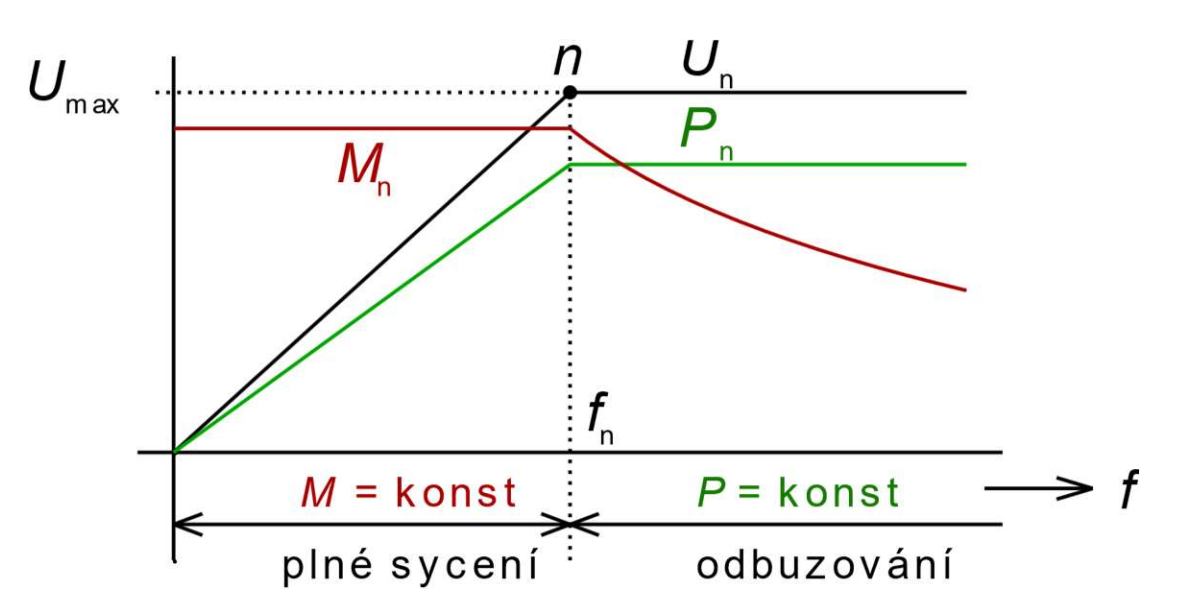
\includegraphics[width=1\linewidth]{images/ProvozniRezimyAMSFrekvencnimMenicem}
	\caption{Závislost napětí, momentu a výkonu na frekvenci \cite{SkriptaRizeniOtacekAM}}
	\label{fig:provoznirezimyamsfrekvencnimmenicem}
\end{figure}

V levé části grafu je oblast konstantního momentu s plným sycením motoru. Zde platí podmínka definovaná v rovnici \ref{eq:PodminkaKonstantnihoSyceni} o konstantním spřaženém magnetickém toku ve statoru. Díky tomu je moment na motoru konstantní a postupně motoru roste výkon, který je definovaný jako:
\begin{equation}
	P = M\omega
	\label{eq:vykonmotoru}
\end{equation}
až do maximální hodnoty výkonu která je v bodě $n$ - jmenovitý bod motoru.

Je také dobré podotknout, že levá část grafu nemůže jít takto od nulového napětí (tento graf je spíše idealizovaný případ), ale jde zpravidla od 10\% jmenovité hodnoty napětí, jelikož se musí pokrýt ztráty které vznikají na odporu statorového vinutí $R_S$. \cite{SkriptaRizeniOtacekAM}

V pravé části grafu je oblast konstantního výkonu ve kterém se motor odbuzuje. Zde už není splněna podmínka z rovnice \ref{eq:PodminkaKonstantnihoSyceni} a tak motoru klesá moment. Vzhledem k tomu, že frekvence statorového napětí stále roste, tak rostou stále i otáčky rotoru.

\subsection{Sinamics G120D}
%\purpose{Popsat hlavní parametry frekvenčního měniče - rozsah napájecího napětí, maximální proud, podporovaný komunikační protokoly (Profinet) - nějaký basic info o Sinamics G120D. Tady přidat i to že Sinamics G120D pracuje s asynchronními motory - jaké jsou od Siemens třeba nejčastější?}

Sinamics G120D je decentralizovaný frekvenční měnič designovaný pro buzení motorů od dopravníkových systémů po elektrické monoraily. Slovo decentralizovaný zde znamená, že frekvenční měnič není jeden centralizovaný, ale že je víc menších frekvenčních měničů blízko u motorů, které ovládají. Kvůli tomu má i certifikaci IP65, která zaručuje dostatečnou kvalitu zpracování, aby bylo možné mít tento frekvenční měnič v náročných prostředí skladů zákazníků firmy Honeywell.
\cite{SinamicsG120D}

Frekvenční měnič obsahuje funkce jako je přesné nastavení polohy motoru, bezpečnostní funkce a dobře konfigurovatelné digitální a analogové vstupy a výstupy. Je to standardní frekvenční měnič který je používán v různých aplikacích hlavně firmami které fungují jako systémoví integrátoři. Běžná podoba tohoto frekvenčního měniče (s kontrolním panelem CU240D-2) je na obrázku \ref{fig:sinamics_G120D}.
\cite{SinamicsG120D}

\begin{figure}[hptb]
	\centering
	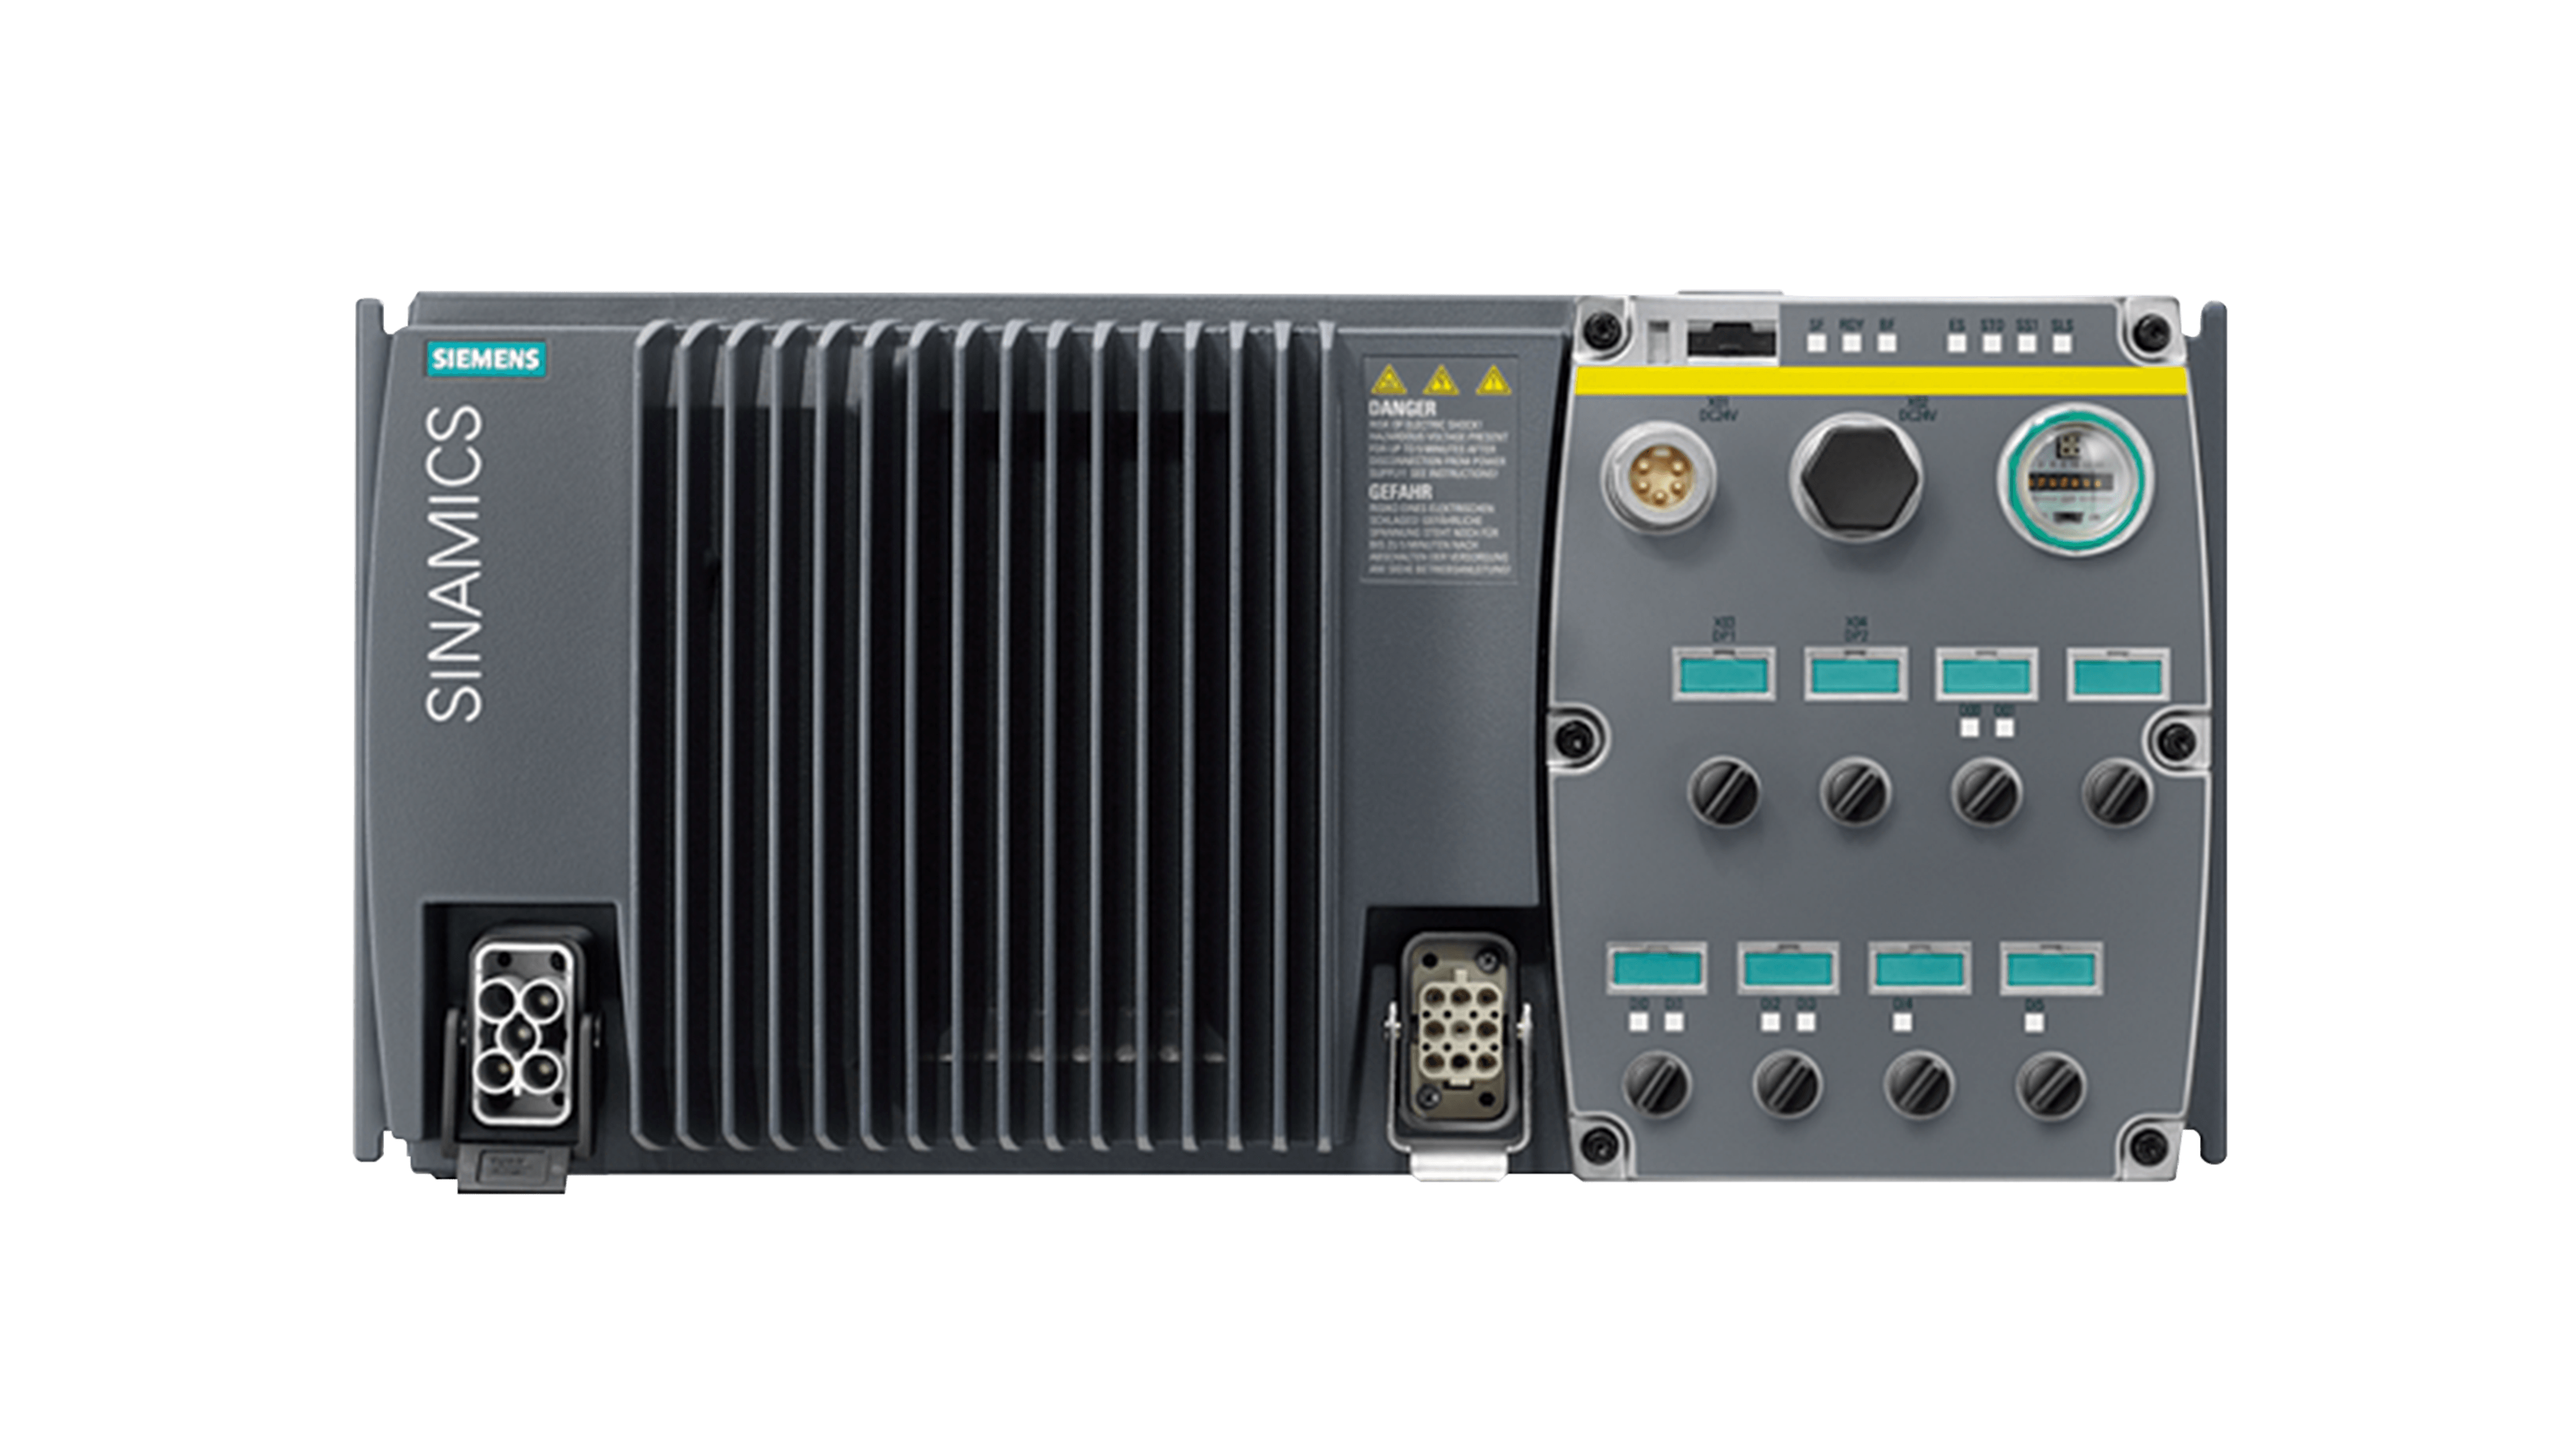
\includegraphics[width=0.8\linewidth]{images/Sinamics_G120D.png}
	\caption{Frekvenční měnič Sinamics G120D \cite{SinamicsG120D}}
	\label{fig:sinamics_G120D}
\end{figure}

Sinamics G120D se v rámci systémů společnosti Siemens dá používat s třífázovými asynchronními motory řad Simotics GP (General Purpose) a Simotics SD (Severe Duty). Jak už název napovídá tak v případě společnosti Honeywell je jako motor nejčastěji používán Simotics GP. Napájecí napětí frekvenčního měniče je také třífázové od $380V$ do  $500V$ dle konfigurace motoru a frekvenční měniče se vyrábí s výkonem $0,75kW$ až $7,5kW$.

Tento frekvenční měnič je tvořen dvěma hlavními částmi - výkonová část a ovládací panel. Ovládací panel ovládá a monitoruje výkonovou část frekvenčního měniče pomocí několika kontrolních systémů na bází uzavřených smyček a díky tomu může kontrolovat bezpečný stav frekvenčního měniče a taky znemožnit ovládání, pokud by s měničem bylo něco v nepořádku. Také je schopný rekuperace energie z brždění linek a vracet ji do sítě, což zákazníkům snižuje náklady na provoz.
\cite{SinamicsG120D}

Všechny tyto funkcionality je možné ovládat přes průmyslové sběrnice PROFINET, PROFIBUS anebo běžnou sběrnicí EtherNet. Tímto způsobem dává PLC příkazy frekvenčnímu měniči v běžném režimu ovládání dopravníků.

\subsection{Nastavení ovládacího panelu}\label{sec:NastaveniOvladacihoPanelu}
%\purpose{Vysvětlit jak se dají dopravníky nastavit aby fungovaly s mým systémem}

Jak bylo dříve zmíněné frekvenční měnič má vždy nějaký ovládací panel. V případě Honeywell instalací je ovládací panel většinou typu Sinamics CU240D-2. Ovládací panely tohoto typu lze za chodu seřizovat třemi způsoby (zobrazené i v obrázku \ref{fig:cu240comissioning}):
\begin{itemize}
	\item Připojení USB z notebooku
	\item Použití PROFINET nebo PROFIBUS
	\item Použití zařízení IOP-2 Handheld
\end{itemize}

\begin{figure}[hptb]
	\centering
	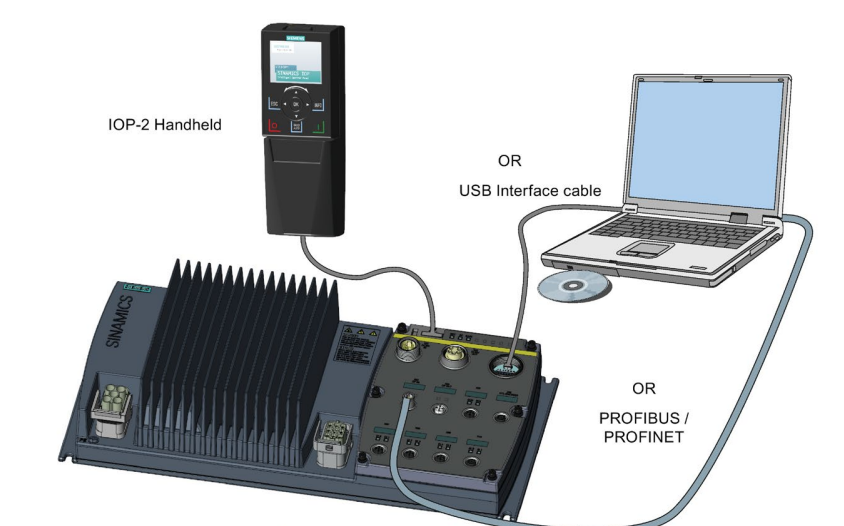
\includegraphics[width=0.7\linewidth]{images/CU240comissioning}
	\caption{Způsoby seřizování ovládacího panelu frekvenčního měniče \cite{SiemensG120DGettingStarted}}
	\label{fig:cu240comissioning}
\end{figure}

Vzhledem k předpokladu, že navrhovaný systém mají používat osoby, které nejsou inženýři specializovaní na kontrolní systémy, je nejvhodnější způsob jak seřizovat ovládací panel použít zařízení IOP-2 Handheld. Ostatní dvě metody vyžadují specializovaný software pro který by bylo zapotřebí instalovat a udržovat si pro něj licence. Naproti tomu IOP-2 Handheld představuje samostatné zařízení schopné provést veškerá potřebná nastavení a je dodáváno s optickým kabelem pro přímé připojení k ovládacímu panelu.

Pro účely navrhovaného systému je potřeba ovládací panel vyresetovat a nastavit do jednoho z  možných výchozích nastavení. Zvolené výchozí nastavení ovlivňuje celý systém, protože ten ovládá dopravník tím, že pomocí relé spíná digitální vstupy ovládacího panelu frekvenčního měniče - tímto způsobem dává systém příkazy na spuštění dopravníku, zrychlení a zpomalení. Nesprávné nastavení ovládacího panelu by vedlo k tomu, že ačkoliv by systém generoval správné signály na digitálních vstupech, panel by je interpretoval chybně.

Navržený systém je optimalizován pro výchozí nastavení číslo 9, ve kterém jsou funkce digitálních vstupů definovány tímto způsobem:
\begin{itemize}
	\item Digitální vstup 0: ON/OFF dopravníku
	\item Digitální vstup 1: Zrychlení dopravníku
	\item Digitální vstup 2: Zpomalení dopravníku
	\item Digitální vstup 3: Kvitování chyby
\end{itemize}
Systém bude konektory připojený k ovládacímu panelu a pomocí relé na desce plošných spojů bude ovládat dopravník rozpojování a zkratováním těchto digitálních vstupů. Digitální vstup č. 3 nebude v rámci systému využíván, protože kvitování případných chyb je vyžadováno pouze jednorázově při resetování do výchozích nastavení a lze jej provést přímo pomocí zařízení IOP-2 Handheld.
\cite{SiemensG120DGettingStarted}.

Resetování ovládacího panelu do tohoto výchozího nastavení je možné provést přímo na místě pomocí zařízení Sinamics IOP-2 Handheld. Pro resetování stačí pouze připojit IOP-2 k ovládacímu panelu frekvenčního měniče, vybrat možnost pro zresetování nastavení ovládacího panelu a vybrat výchozí nastavení číslo 9. Zbytek hodnot na ovládacím panelu, jako je například zrychlující rampa, může zůstat na výchozích hodnotách, protože je není potřeba v rámci testování kvality instalace mít na správných hodnotách (frekvenční měnič funguje i tak). Poté je možné odpojit IOP-2 od ovládacího panelu, který tímto způsobem zůstane nastavený nadále.



\subsubsection{Alternativní výchozí nastavení ovládacího panelu}
%\purpose{popsat nastavení default with potentiometer a default MOP with E-STOP}

Při návrhu systému byla kromě výchozího nastavení číslo 9 zvažována i další relevantní výchozí nastavení, konkrétně nastavení č. 8 a č. 12.

Výchozí nastavení č. 8 by definovalo chování systému následovně:
\begin{itemize}
	\item Digitální vstup 0: ON/OFF dopravníku
	\item Digitální vstup 1: Zrychlení dopravníku
	\item Digitální vstup 2: Zpomalení dopravníku
	\item Digitální vstup 3: Kvitování chyby
	\item Digitální vstup 4: Při přerušení nouzově zastaví (E-STOP)
	\item Digitální vstup 5: Při přerušení nouzově zastaví (E-STOP)
\end{itemize}
Tohle výchozí nastavení nabízí stejnou funkcionalitu jako zvolené nastavení č. 9, ale vyžaduje připojení dalšího kabelu na kterém bude v obvodu umístěné bezpečnostní tlačítko E-STOP, které by také muselo mít dostatek místa ve schránce systému. Tohle výchozí nastavení bylo zamítnuto právě kvůli tomu, že E-STOP tlačítko vyžaduje neúměrně příliš mnoho místa a tak by to výrazně zvětšilo rozměry systému, což by zmenšovalo přenositelnost a jednoduchost používání. Bezpečnost systému je přitom zajištěna jinými bezpečnostními prvky přímo u dopravníků, jak je podrobněji popsáno v kapitole \ref{sec:PosouzeniZHlediskaBezpecnosti}.
\cite{SiemensG120DGettingStarted}

Další zvažovanou alternativou bylo výchozí nastavení č. 12, které by definovalo funkce vstupů takto:
\begin{itemize}
	\item Digitální vstup 0: ON/OFF dopravníku
	\item Digitální vstup 1: Reverzace směru otáčení
	\item Digitální vstup 2: Kvitování chyby
	\item Analogový vstup: Nastavení rychlosti
\end{itemize}
Toto nastavení by umožnilo připojení potenciometru k analogovému vstupu ovládacího panelu pro přímé nastavení rychlosti. Díky tomuto by bylo o jedno tlačítko méně na schránce systému, ale zároveň by to vyžadovalo speciální kabely pro připojení (vzhledem k tomu, že se analogové vstupy ovládacích panelů v instalacích Honeywell běžně nevyužívají) a také by to zahrnovalo modifikaci desky plošných spojů, například s využitím integrovaného obvodu digitálně řízeného potenciometru.
\cite{SiemensG120DGettingStarted}

Po zhodnocení těchto možností bylo vybráno výchozí nastavení č. 9.

\subsection{Bezpečnostní aspekty práce s ovládacím panelem}
%\purpose{Zmínit že když pracuji s takovýmto výkonovým zařízením, musím si dát pozor na bezpečnost. Vysoký napětí který vystupuje z frekvenčního měniče se dá vypnout přepínačem který je umístěný nad ovládacím panelem. Potom už člověk pracuje jen s 24V které jsou na všech portech ovládacího panelu a kvůli tomu všechny porty zakrývají šroubovací gumové kryty, které je potřeba oddělat předtím než se můžou připoji kabely ze systému co navrhuji.}

Vzhledem k tomu, že frekvenční měnič pracuje ve výkonové části s usměrněným trojfázovým napětím, je velmi důležité dbát na bezpečnost při práci s frekvenčním měničem. Z tohoto důvodu je vedle každé instalace frekvenčního měniče v Honeywell umístěn bezpečnostní vypínač, který vypojuje napájení výkonové části frekvenčního měniče. Pro bezpečné zacházení s frekvenčním měničem je potřebné mít tento vypínač ve stavu rozpojeno.

Po rozpojení napájení výkonové části zůstává na ovládacím panelu napětí $24V$. Tohle nízké napětí je ale chráněno šroubovacími gumovými krytkami, které zakrývají veškeré digitální vstupy a výstupy ovládacího panelu kde se toto napětí nachází.

\section{Open-source vývojové desky ($\Sigma$ = 2.5 strany)}
%\purpose{Zde bude úvod do open source vývojových desek.}

Mikrokontroller, mozek praktické části bakalářské práce, není integrován přímo na desce s výkonovou částí zařízení. Využita byla možnost open-source vývojové desky, přičemž toto označení je dnes často synonymem pro Arduino, značku s největším přínosem v této oblasti.

Myšlenka vývojových desek jako jsou Arduino desky začala myšlenkou minimalismu - desky nebyly nikdy převratné, ale obsahovaly přesně to, co je potřeba. Na jedné vývojové desce je obsažený mikrokontroller, převodník z USB do sériové komunikace a dle desky obsahuje další užitečné součástky. Je zde možné tedy nejenom využívat periferie použitého mikrokontrolleru, ale i další hardware, jako jsou externí krystaly, napájení mimo USB kabel a další na základě specifického návrhu vývojové desky.
\cite{KnihaOArduinu}

Rychlou adaptaci veřejností umožnil nejenom kvalitní design desek, ale i software pro programování Arduino desek na počítači. Na rozdíl od předchozího proprietárního softwaru, který nebyl dostupný pro všechny operační systémy, je programovací prostředí Arduina open-source a spustitelné na všech systémech s podporou Java aplikací.
\cite{KnihaOArduinu}

Kromě výhod ekosystému Arduino existují obecné důvody pro použití hotových vývojových desek namísto přímé integrace mikrokontrolleru v prototypování a vývoji. Mezi hlavní výhody patří možnost připojení vývojové desky pomocí kolíkových lišt, což umožňuje snadné vyjmutí pro přeprogramování nebo výměnu. Přímá integrace by v případě poruchy vyžadovala odpájení. Díky tomu vývojová deska celkově usnadňuje prototypování a opravitelnost.

Nakonec je důvodem zvolení open source vývojových desek do systému i jejich dostupnost a flexibilita kterou nabízejí. Jelikož jsou schémata zapojení desek veřejně dostupná, může je vyrábět jakýkoliv výrobce. Navíc je také možné používat veřejně dostupná schémata zapojení desek při návrhu vlastních desek plošných spojů do kterých jsou vývojové desky integrované a díky tomu známá přesná propojení jednotlivých komponentů v celé navržené desce plošných spojů.

\subsection{Proč WEMOS vývojové desky (1 strana)}
%\purpose{Tady bude popsané co jsou WEMOS desky a proč je používám. Taky tady bude důvod proč jsem si vybral WEMOS D1 Mini pro a srovnání s wemos D1 mini a arduino UNO}

Arduino v dnešní době není jediná firma, která vyrábí open-source vývojové desky. Pro tuhle bakalářskou práci byla zvolena vývojová deska od společnosti WEMOS, která je výrobce vývojových desek které jsou podobné Arduino deskám, ale jejich zaměření je specificky ve vytváření kompaktních desek které mají integrovanou bezdrátovou konektivitu (WiFi a bluetooth) pomocí populárních mikrokontrolérů ESP32 a ESP8266 od společnosti Espressif Systems.

Mít možnost používat WiFi je důležitý požadavek, který musí vývojová deska splňovat. Pokud bude systém možné ovládat přes WiFi, je možné pro ovládání použít jakékoliv zařízení, které má WiFi technologii, což je v dnešní době většina chytrých zařízení. Kvůli tomu lze dopravník ovládat širokým spektrem chytrých zařízení a tak není potřeba aby s sebou uživatelé nosili dedikovaný vysílač.

Společnost WEMOS nabízí několik modelů vývojových desek s různými mikrokontroléry a periferiemi. Mezi známé varianty patří například:
\begin{itemize}
	\item \textbf{WEMOS D1 Mini:} Kompaktní deska postavená na mikrokontroléru ESP8266EX. Poskytuje 11 digitálních GPIO pinů (z toho 10] s podporou PWM a podporou přerušení), 1 analogový vstup, I2C rozhraní, 4MB Flash paměti a integrovanou PCB anténu pro WiFi. Napájení a programování se provádí přes USB-C konektor. Deska je oblíbená pro své malé rozměry a širokou podporu, ale omezuje ji malý počet GPIO pinů, což desku nedělá dobrou pro prototypování nebo rozsáhlejší aplikace.
	\item \textbf{WEMOS C3 Mini:} Novější varianta využívající mikrokontrolér ESP32-C3. Tento čip integruje WiFi i Bluetooth konektivitu. Deska disponuje USB-C konektorem, 4 MB Flash paměti a 12 GPIO pinů.
\end{itemize}

Tenhle systém je ale navrhován pro industriální prostředí a je velmi důležité aby byla bezdrátová komunikace co nejspolehlivější. Proto je potřebné mít na vývojové desce k dispozici externí anténu, která významně zvýší dosah WiFi komunikace díky lepšímu umístění antény. Proto byla do systému vybrána vývojová deska WEMOS D1 Mini Pro kterou lze vidět na obrázku \ref{fig:WEMOSD1MiniPro}. Tato deska sdílí většinu vlastností s modelem D1 Mini, ale narozdíl od levnějšího modelu má 16MB Flash paměti, které jsou také velmi důležité vzhledem k tomu, že na kód pro systém by 4MB Flash paměti nestačilo.

Všechny vývojové desky WEMOS s mikrokontroléry ESP8266 a EPS32 lze programovat pomocí prostředí Arduino IDE (nebo alternativy jako PlatformIO) s využitím Arduino jazyka založeného na C++, nebo alternativně pomocí MicroPython. Celá aplikace je programována pomocí Arduino framework pro ESP8266. Webové ovládání je prováděno pomocí knihovny WebServer, která umožňuje běh nenáročných síťových aplikací (více je popsané v kapitole \ref{sec:ArduinoFrameworkForESP8266}).

\begin{figure}[hptb]
	\centering
	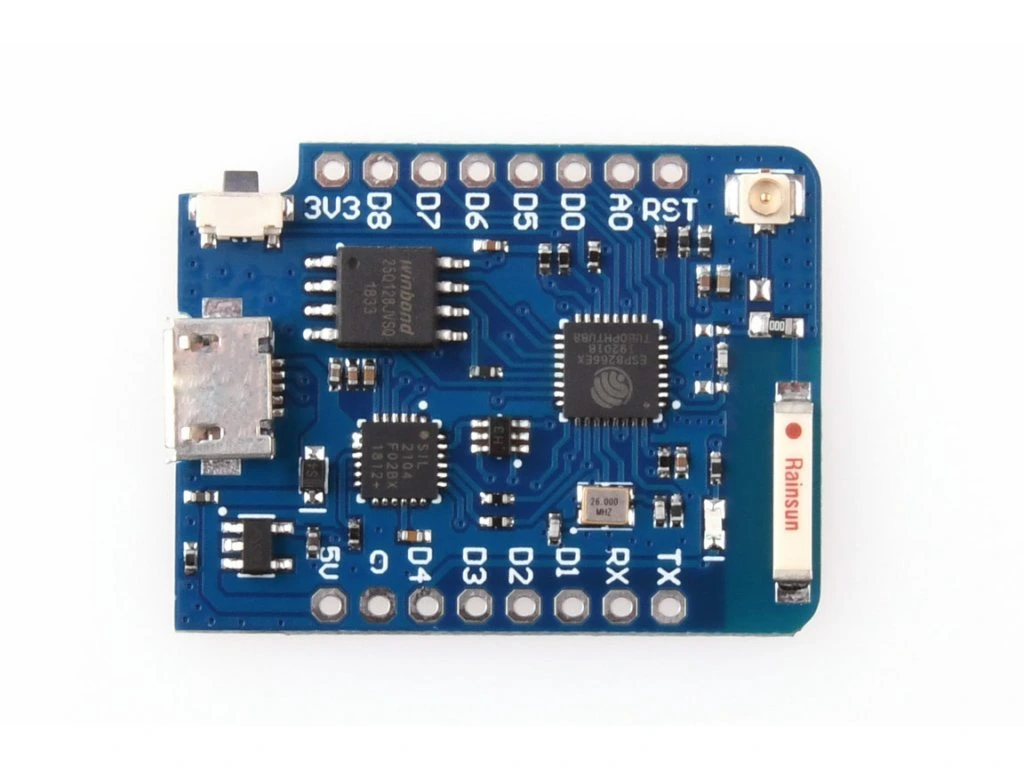
\includegraphics[width=0.8\linewidth]{images/WEMOS_D1_Mini_Pro.png}
	\caption{Použitá varianta vývojové desky WEMOS D1 Mini Pro \cite{WEMOSD1MiniPro}}
	\label{fig:WEMOSD1MiniPro}
\end{figure}

\subsection{Technické specifikace WEMOS D1 Mini Pro (1.5 strany)}
% \purpose{Rozvinout co jsou specifikace D1 Mini Pro a co ty jednotlivé věci znamenají - počet GPIO, I2C, PWM, paměť, typ mikrokontrolleru, atd. - nějaký základní basic informace}

Na základě požadavků projektu a srovnání s alternativami je pro realizaci hardwarového návrhu nejefektivnější vývojová deska WEMOS D1 Mini Pro. Tato sekce popisuje její technické parametry s jejich využitím v návrhu. Samotná deska je postavena na mikrokontroléru ESP-8266EX a je velmi kompaktní, zatímco ale stále poskytuje dost funkcionalit a vstupních a výstupních pinů pro provoz zařízení.

Technické specifikace této vývojové desky jsou následující: \cite{ESP8266EXDatasheet, D1MiniProDokumentace}
\begin{itemize}
	\item Mikrokontrolér: ESP-8266EX
	\item Napájecí napětí: $5V$
	\item Provozní napětí: $3,3V$
	\item Počet digitálních I/O pinů (GPIO): 11. Tyto piny slouží pro digitální vstupní a výstupní signály které budou ovládat dopravník a na základě kterých se bude aproximovat rychlost dopravníku.
	\item Podpora periferií na GPIO pinech: Většina digitálních pinů podporuje funkce jako:
	\begin{itemize}
		\item Přerušení (Interrupt): Umožňuje reakci mikrokontroléru na externí události.
		\item PWM (Pulse Width Modulation): Pro generování semi-analogového signálu nebo snížení střední hodnoty napětí. Až 10 pinů má podporu PWM.
		\item I2C: Dvouvodičová sériová sběrnice používaná pro komunikaci s periferiemi, jako je v tomto projektu použitý LCD displej. Deska disponuje dedikovanými piny pro tuto sběrnici na pinech D1 a D2.
		\item One-wire: Sériová sběrnice pro komunikaci s některými typy senzorů.
	\end{itemize}
	\item Analogový vstupní pin: 1. Tento pin umožňuje měřit analogové napětí, například z některých typů senzorů. Maximální vstupní napětí pro tento pin je 3.2V.
	\item Paměť:
	\begin{itemize}
		\item Flash paměť: 16 MB. Tato velká kapacita Flash paměti je důležitá pro uložení aplikačního kódu, rozšiřujících knihoven (jako je WebServer) a webových souborů co jsou hostované na serveru.
		\item RAM: 50 kB. Slouží pro běh programu a ukládání proměnných.
	\end{itemize}
	\item Bezdrátová konektivita: Integrovaná WiFi na frekvenci 2.4 GHz.
	\item Anténa: Možnost připojení externí antény prostřednictvím IPEX1 / SMA konektoru nebo využití vestavěné keramické antény pro testování. Pro zvýšení spolehlivosti a dosahu v industriálním prostředí je využita možnost externí antény.
	\item Napájení a programování: Micro USB konektor. Deska může být napájena přes USB nebo přes 5V pin.
	\item Napájení z baterie: Rozhraní pro připojení lithiové baterie s nabíjecím proudem až 500mA. Toto rozhraní ale v tomto projektu není využíváno a navržená deska plošných spojů není pro používání baterie uspořádána.
	\item Kompatibilita: Deska je kompatibilní s vývojovými prostředími a firmwary jako Arduino, MicroPython a NodeMCU, což poskytuje flexibilitu při vývoji firmwaru.
\end{itemize}

Zapojení vývojové desky do navrhnuté desky plošných spojů je popsáno v kapitole \ref{sec:Hardware}.

\subsection{Arduino framework pro ESP8266}\label{sec:ArduinoFrameworkForESP8266}
% \purpose{Trochu uvést do kontextu jak funguje arduino framework for esp8266 a jak specificky řeším provozování webserveru na mým MCU.}

Pro programování mikrokontrolerů z řad EPS8266 je možné využít jejich nativního software development kitu (SDK) anebo takzvaný "Arduino framework" pro tuto platformu. Tato knihovna je portace SDK pro platformu Arduino a díky tomu je možné používat prostředí jako je Arduino IDE nebo Platformio pro programování ESP8266 mikrokontrolerů. Tohle všechno je možné i přesto, že mají ESP8266 i Arduino přirozeně různé základy, které spolu ve výchozím stavu nejsou kompatibilní. Tato podpora umožňuje velkému množství hobby i profesionálním programátorům programovat ESP8266 mikrokontrolery ve stejném prostředí jako ve kterém programovali své Arduino projekty. To všechno bez ztráty hardwarových nebo síťových periferií.

"Arduino framework pro ESP8266 je podpora ESP8266 mikrokontroleru pro Arduino prostředí. To vývojářům umožňuje používat známé Arduino funkce a knihovny, které je možné spouštět přímo na ESP8266 mikrokontrolleru." \cite{ESP8266ArduinoFrameworkGithub}

V této práci byl kód mikrokontroleru programován uvnitř programovacího prostředí PlatformIO (ukázané na obrázku \ref{fig:PlatformioUkazka}) ve kterém byl Arduino framework pro ESP8266 využitý. Byla využitá i kompatibilita s existujícími Arduino knihovnami, jako v případě knihovny Ticker. To je knihovna, která v rámci Arduino zařízení umožňuje nastavit časovač, který spouští některou funkci pravidelně přesné časové intervaly.

\begin{figure}[hptb]
    \centering
    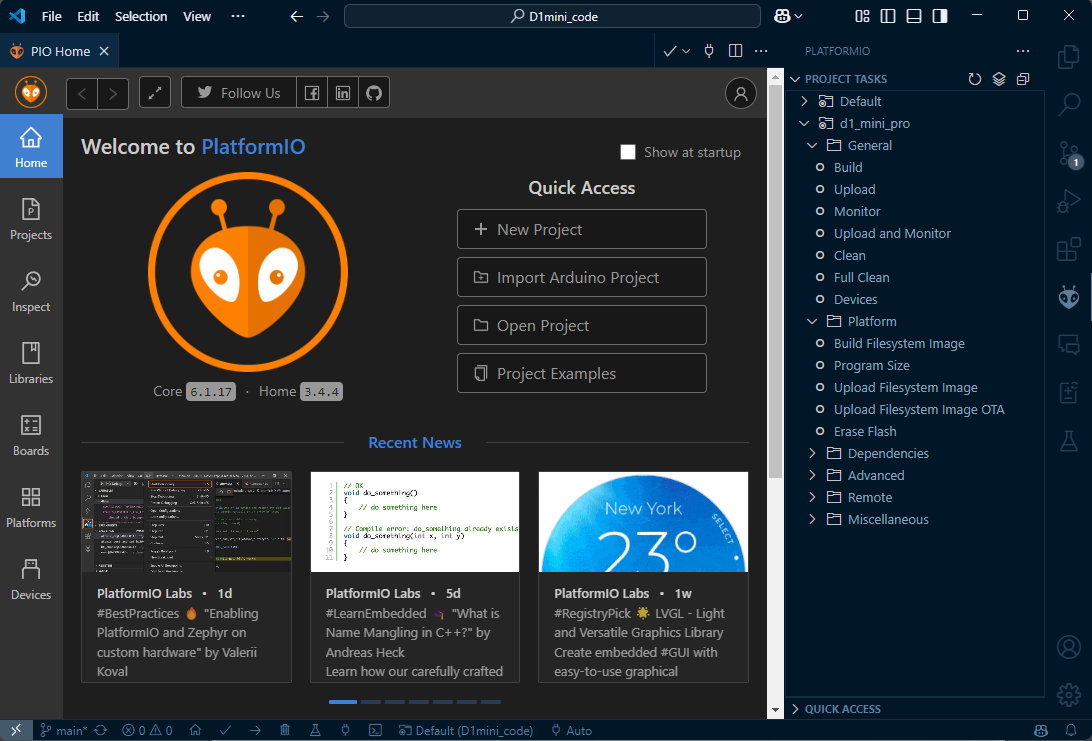
\includegraphics[width=0.9\linewidth]{images/Platformio_Ukazka.png}
    \caption{Ukázka rozhraní vývojového prostředí Platformio}
    \label{fig:PlatformioUkazka}
\end{figure}

\subsubsection{Knihovny pro webové funkce}
%\purpose{Popsat co dělají knihovny ESP8266WiFi, WiFiClient, ESP8266WebServer a ESP8266mDNS}

Využití Arduino frameworku pro ESP8266 plně umožňuje využít i WiFi funkcionality tohoto mikrokontroleru. Knihovny co jsou využité jsou knihovny ESP8266WiFi, ESP8266WebServer a ESP8266mDNS.

Knihovna \textbf{ESP8266WiFi} je základní stavební kámen veškeré síťové komunikace. Bez této knihovny by se mikrokontroler nemohl připojit k existující bezdrátové síti nebo si vytvořit vlastní hotspot. V kódu se implementuje pomocí příkazů jako je \textit{WiFi.begin(jmeno,heslo)}.

Funkcionalitu web serveru, která je velmi důležitá pro tento projekt implementuje knihovna \textbf{ESP8266WebServer}. Tato knihovna poskytuje funkce pro definování plně funkčního HTTP serveru a odpovědi na jeho webové požadavky (např. GET pro získání dat, POST pro doesílání dat a další). Tento webový server umí servírovat statické webové stránky, ale umí v rámci jejich provádění i spouštět jakékoliv další funkce mikrokontroleru. Tohle umožňuje ovládat mikrokontroler skrz odpovědi na webové adresy.

Knihovna \textbf{ESP8266mDNS} neboli ESP8266 multicast DNS je knihovna, který umožňuje ukládat IP adresu mikrokontroleru na jakýchkoliv předem definovaných adresách která stačí zadat do prohlížeče na zařízení, které má server mikrokontroleru k dispozici.

Tyto tři knihovny se dohromady dají nastavit například tak, aby se pomocí jedné webové stránky dostupné na IP adrese \textit{espwebserver} dala ovládala LED dioda na mikrokontroleru.

\begin{figure}[H]
	\centering
	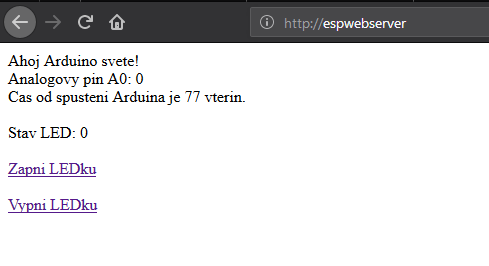
\includegraphics[width=0.7\linewidth]{images/ESPWebserverUkazka}
	\caption{Ukázka nastavení WebServeru pro ovládání LED diody \cite{NavodNaESPWebServerDratek}}
	\label{fig:espwebserverukazka}
\end{figure}

\begin{lstlisting}[language=C++, caption={Nastavení ESP8266 WebServeru pro ovládání LED diody \cite{NavodNaESPWebServerDratek}}, label={lst:NastaveniWebServeru}]
	#include <ESP8266WiFi.h>
	#include <ESP8266WebServer.h>
	#include <ESP8266mDNS.h>

	const char* nazevWifi = "Ardwifi";
	const char* hesloWifi = "arduino1234";

	ESP8266WebServer server(80);

	#define LEDka LED_BUILTIN
	#define analogPin A0

	void zpravaHlavni() {
		String analog = String(analogRead(analogPin));
		String cas = String(millis() / 1000);
		String ledStatus = digitalRead(LEDka) ? "ZAPNUTO" : "VYPNUTO";

		String zprava =
		"<h1>ESP8266 WebServer</h1>"
		"Hodnota analogoveho pinu A0: " + analog + "<br>"
		"Cas od spusteni: " + cas + " vterin.<br><br>"
		"Stav LED (pin " + String(LEDka) + "): " + ledStatus + "<br><br>"
		"<a href=\"/ledON\">Zapni LEDku</a><br>"
		"<a href=\"/ledOFF\">Vypni LEDku</a>";

		server.send(200, "text/html", zprava);
	}

	void setup() {
		pinMode(LEDka, OUTPUT);
		digitalWrite(LEDka, LOW);

		WiFi.begin(nazevWifi, hesloWifi);

		while (WiFi.status() != WL_CONNECTED) {
			delay(50);
		}

		MDNS.begin("espwebserver");

		server.on("/", zpravaHlavni);
		server.on("/ledON", []() {
			digitalWrite(LEDka, HIGH);
			zpravaHlavni();
		});
		server.on("/ledOFF", []() {
			digitalWrite(LEDka, LOW);
			zpravaHlavni();
		});

		server.begin();
	}

	void loop() {
		server.handleClient();
		\delay(10)
	}
\end{lstlisting}

V ukázce kódu \ref{lst:NastaveniWebServeru} lze z webových funkcionalit vidět hlavně globální objekt typu ESP8266WebServer s názvem server, pomocí kterého lze odpovídat na webové požadavky definované ve funkci \textit{setup()}. Funkce \textit{zpravaHlavni} je funkce kterou se odpovídá na většinu webových GET požadavků a tak je lépe definovaná a obsahuje dodatečné informace o stavu LED diody a času od spuštění. Tato funkce také rovnou obsahuje kód v jazyce HTML, ve kterém se píšou webové stránky.

Kód dále obsahuje připojení na WiFi pod zadaným názvem a heslem s tím že čeká na připojení a až poté bude provádět zbytek kódu. Zbytek \textit{setup()} funkce obsahuje odpovědi na webové požadavky. Každá odpověď na webový požadavek odpoví tím, že zpět pošle HTML kód z funkce \textit{zpravaHlavni} (který zobrazuje informace jako jsou v obrázku \ref{fig:espwebserverukazka}), ale v případě adres \textit{/ledON} a \textit{/ledOFF} stránka ještě nastaví vysokou nebo nízkou hodnotu na LED diodu na vývojové desce.

Nakonec je zde funkce \textit{loop()}, která se každých 10 milisekund snaží odpovídat na webové požadavky. Na základě zadaných adres odpovídá prováděním bloků kódu které byly nastaveny v \textit{setup()} funkci.

% Na doporučení vedoucího tyhle kapitoly už nedělám, protože se budu moct lépe vyřádit v té praktické části
%\subsubsection{Architektura ESP8266EX}
%\purpose{Vysvětlit jaké jsou parametry ESP8266 a proč se ESP8266 víc hodí pro tento projekt než ESP32.  ESP32 má wifi i bluetooth a ESP8266 má jen wifi. Zdroj needed.}
% Myslím si že je to navíc. Až tak dohloubky jsem to neřešil, protože mě hlavně zajímaly ty parametry mojí vývojové desky.

%\subsection{Arduino jazyk a Platformio (3 strany)}
%\purpose{Vysvětlení že existuje arduino jazyk a na čem je založen, zmínění že existuje Arduino IDE a vysvětlení základu jak funguje platformio a jak se liší od Arduino IDE.}
%
%\purpose{Vysvětlení že existují soubory funkcí a hlavičkové soubory.}
%
%\source{Tady možná budu muset mít internetový zdroje, protože jsem nenašel žádnou publikaci co by mluvila o Platformio.}
%
%
%\subsubsection{Objekty v arduino C++ jazyce}
%\purpose{Tady bych rád vysvětlil jak fungují objekty v arduino C++ jazyce jelikož je využívám uvnitř kapitoly \ref{sec:ConveyorController}. }
%
%U objektů jde obecně jde hlavně o to, že si můžu vytvořit globální instanci objektu a tam si zadefinovat public metody a public proměnné (které můžu zavolat a získat přímo z objektu a používat v main kódu) a private metody a private proměnné (které jsou dostupné jenom uvnitř objektu, takže je můžu získat jen vevnitř jiných metod a proměnných).
%
%\subsubsection{Ticker knihovna}\label{sec:TickerKnihovna}
%\purpose{Podobně jako existuje timer u microchip MCU existuje i timer knihovna zvaná Ticker u MCU co se programují v arduino jazyce. Tuhle knihovnu já používám a zmiňuju v sekci \ref{sec:ImplementaceConveyorControllerVeMainCpp} a tak se hodí ji trochu vysvětlit.}
%
%Vývojové desky kompatibilní s platformou Arduino umožňují integraci knihovny Ticker, která poskytuje mechanismus načasování funkcí v definovaných intervalech bez blokování provádění zbytku kódu. Pokud by byla použita funkce \texttt{delay()}, mohlo by to vést ke dvěma problémům. Prvním je různý čas délky vykonávání kódu, které by zesložiťovala spolehlivé nastavení přesných časových intervalů. Druhým problémem je blokující povaha funkce \texttt{delay()}, která by znemožnila časově kritické operace, jako je například reakce na síťové požadavky na serveru nodeMCU běžícím na mikrokontrolrru, což by mohlo zpomalit funkčnost celého systému. \cite{TickerKnihovna}
%
%Je tedy možné se spolehnout na to, že se bude prováděná funkce spouštět přesně ve stanovený čas, což umožňuje aproximaci rychlosti dopravníku která je popsána v kapitole \ref{sec:AproximaceRychlostiDopravniku}.
%
%Pro použití Ticker knihovny je potřebné si knihovnu nejdříve importovat pomocí příkazu \texttt{\#include "Ticker.h"} v záhlaví souboru a následně je možné ji nastavit v \texttt{setup()} funkci hlavního skriptu.
%
%\begin{lstlisting}[language=C++, caption={Použití ticker knihovny uvnitř \texttt{setup()} funkce \cite{TickerGitHubPage}}, label={lst:TickerUkazka}]
%Ticker tickerObject(callbackFunction, 1000); // Zadefinuje ticker objekt
%tickerObject.start(); //Spusti Ticker.
%\end{lstlisting}
%kde je \texttt{callbackFunction} je funkce která bude provedena při každém spuštění Ticker objektu.
%
